%% LyX 2.0.3 created this file.  For more info, see http://www.lyx.org/.
%% Do not edit unless you really know what you are doing.
\documentclass[usenatbib]{mn2e}
\usepackage[latin9]{inputenc}
\usepackage[a4paper]{geometry}
\geometry{verbose}
\setcounter{tocdepth}{3}
\usepackage{color}
\usepackage{float}
\usepackage{graphicx}

\makeatletter

%%%%%%%%%%%%%%%%%%%%%%%%%%%%%% LyX specific LaTeX commands.
%% Because html converters don't know tabularnewline
\providecommand{\tabularnewline}{\\}
%% A simple dot to overcome graphicx limitations
\newcommand{\lyxdot}{.}


%%%%%%%%%%%%%%%%%%%%%%%%%%%%%% User specified LaTeX commands.






%%%%%%%%%%%%%%%%%%%%%%%%%%%%%% LyX specific LaTeX commands.
%% A simple dot to overcome graphicx limitations
%Make my life significantly easier

\global\long\def\bd{{\bm{\delta}}}

\makeatother

\begin{document}
We are interested in recovering the halos and their masses, positions
and velocities with the smallest time step necessary to preserve sufficient
properties as mock catalogs.


\section{Matching Halos}

First, we compare a halo by halo in different simulations. Since all
the simulations use exactly the same initial conditions, if those
approximated N-body simulations can recover the halos reasonably well
(compared to a full N-body simulation), then we should find the same
halo at the same position with the same mass in samples using different
mass resolutions and time steps. The question here are how mass resolutions
and time steps affect on halo properties (i.e., mass, position and
velocity) and how many halos don't correspond to halos between different
samples.

To spatially match the halos defined in different simulations, we
first find a pair of halos from two different simulations, whose distance
is the closest. Then, we set two conditions on those pairs to declare
whether those paired halos are the same halos:

1) distance is smaller than $0.5h^{-1}{\rm Mpc}$,

2) mass ratio is smaller than $10^{0.5}{\rm M_{\odot}}$.

Under the above conditions, \textcolor{black}{more than}\textcolor{red}{{}
}90\% of halos in 450/5 found paired halos in 300/2 at redshift $z=0.15$
with a fixed mass resolution, $256^{3}$ particles (shown in \textcolor{black}{Table}\textcolor{red}{{}
}\ref{tab:unmatchedHalo}). Both simulations have the same mass resolution,
which is a $256^{3}$ particles in a $256^{3}(h^{-1}{\rm Mpc})^{3}$
cubic box. We also checked how those conditions affect to fraction
of matched halos by changing the numerical values for distance and
mass ratio criteria. As shown in Table \ref{tab:unmatchedHalo}, changing
a criterion on mass ratio did not change the fraction much, while
the distance conditions does. This iimplies that deviation of halo
masses on pairs is relatively small.

\begin{table*}[p]
\begin{tabular}{|c|c|c|c|}
\hline 
mass$[{\rm M_{\odot}]}$\textbackslash{}distance $[h^{-1}{\rm Mpc}]$ & 0.5 & 0.75 & 1.0\tabularnewline
\hline 
\hline 
$10^{0.5}$ & 0.0915 & 0.0842 & 0.0842\tabularnewline
\hline 
$10^{0.75}$ & 0.0909 & 0.0825 & 0.0817\tabularnewline
\hline 
$10^{1.0}$ & 0.0909 & 0.0823 & 0.0763\tabularnewline
\hline 
\end{tabular}

\caption{\label{tab:unmatchedHalo}Fractions of unmatched halos (over matched
halos) for the sample of 450/5 when we compare a halo by halo for
300/2 at redshift $z=0.15$. Here, both simulations have the same
mass resolution (i.e., $256^{3}$ particles in the box of $(256h^{-1}{\rm Mpc})^{3}$).
This table shows how the fraction is changed according to changing
the matching conditions for distance and mass ratio.}


\end{table*}



\subsection{Mass Resolution}

In this section, we examine how mass resolutions affect to halo properties.
We use a $(256h^{-1}{\rm Mpc)^{3}}$-cubic box and three different
mass resolutions: $512^{3}$, $256^{3}$, and $128^{3}$ particles
with a fixed time steps (450/5). We take a simulation of $512^{3}$
particles as a reference. Table \ref{tab:unmatched_512} indicates
fractions of unmatched halos in the sample of $512^{3}$-particle
mass resolution by matching with the samples of $256^{3}$ and $128^{3}$
particles. Since having a different mass resolution implies that halo
samples have different lower mass limits, we only impose matching
conditions on halos greater than $10^{12.5}{\rm M_{\odot}}$ for the
case of $256^{3}$-particles sample and greater than $10^{13.5}{\rm M_{\odot}}$
for the case of $128^{3}$-particles sample. For matching between
$512^{3}$ and $256^{3}$ partciles, the above matching conditions
are enough to find pairs for most of halos. On the other hand, as
indicated in Figure \ref{fig:HaloPosition512}, separations of matched
halos between $512^{3}$ and $128^{3}$ particles are bigger than
$0.5h^{-1}{\rm Mpc}$ and the distance condition it too tight to find
a pair. The right panel in Table \ref{tab:unmatched_512} shows how
unmatched fractions are changed by changing the distance condition.
This suggests that dynamics for $128^{3}$ and $512^{3}$ are very
different(?)...

\begin{table*}[p]
\begin{tabular}{|c|c|c|c|}
\hline 
mass-resolution\textbackslash{}z & 0.15 & 0.5 & 0.8\tabularnewline
\hline 
\hline 
$256^{3}$ & 0.150 & 0.128 & 0.120\tabularnewline
\hline 
$128^{3}$ & 0.842 & 0.831 & 0.817\tabularnewline
\hline 
\end{tabular}%
\begin{tabular}{|c|c|c|c|}
\hline 
z\textbackslash{}distance $[h^{-1}{\rm Mpc}]$ & 0.5 & 1.0 & 2.0\tabularnewline
\hline 
\hline 
0.15 & 0.842 & 0.260 & 0.061\tabularnewline
\hline 
0.5 & 0.831 & 0.260 & 0.066\tabularnewline
\hline 
0.8 & 0.817 & 0.213 & 0.053\tabularnewline
\hline 
\end{tabular}

\caption{\label{tab:unmatched_512}Left: Fractions of unmatched halos (over
matched halos) for the sample of $512^{3}$ particles when we compare
a halo by halo for $256^{3}$ and $128^{3}$ particles with a fixed
time step (450/5). For the comparison between $512^{3}$ and $256^{3}$
particles, we select halos greater than $10^{12.5}{\rm M_{\odot}}$,
while for the case of $512^{3}$ and $128^{3}$ particles, halos greater
than $10^{13.5}{\rm M_{\odot}}$ are selected. Right: For the comparison
between $512^{3}$ and $128^{3}$ particles, we examined how the unmatched
fractions are changed due to distance conditions.}
\end{table*}


\begin{figure*}
\includegraphics[width=1\columnwidth]{/Users/ts485/Dropbox/Tomomi/HACC/Conv/Matching_halos/plots_450_5/unmatchedHalo_256_450_5_z0\lyxdot 15}\includegraphics[width=1\columnwidth]{/Users/ts485/Dropbox/Tomomi/HACC/Conv/Matching_halos/plots_450_5/unmatchedHalo_128_450_5_z0\lyxdot 15}

\caption{\label{fig:unmatchedHalo512}Unmatched halo number density for the
simulation of $512^{3}$ particles (blue in both panels) by comparing
with $256^{3}$ particles-simulation (left, green) and $128^{3}$-particles
simulation (right, green) at redshift $z=0.15$. }
\end{figure*}


Figure \ref{fig:unmatchedHalo512} shows number densities of unmatched
halos as a function of halo mass at redshift $z=0.15$. In matching,
an algorithm takes a finer resolution sample as a reference and finds
a matched halo from the other sample. Surprisingly, the number densities
for bothe samples are almost the same.

\begin{figure*}
\includegraphics[width=1\columnwidth]{/Users/ts485/Dropbox/Tomomi/HACC/Conv/Matching_halos/plots_450_5/distance1_normed_450_5_z0\lyxdot 15}
\includegraphics[width=1\columnwidth]{/Users/ts485/Dropbox/Tomomi/HACC/Conv/NoDist_M14\lyxdot 0_distance1_normed_450_5_z0\lyxdot 15}

\caption{\label{fig:HaloPosition512}Left: Histograms of distance difference
for matched halos with respect to halos from $512^{3}$ particles
with 450 global steps and 5 sub-cycles. Different colors correspond
to different mass resolutions: $256^{3}$ particles and $128^{3}$
particles with a fixed time step (450/5) at redshift $z=0.15$. Right:
Histograms of distance difference for matched halos without iposing
a distance condition. Halos are selected so that their masses are
greater than $10^{14}{\rm M_{\odot}}$ at redshift $z=0.15$.}


\end{figure*}


Figure \ref{fig:HaloPosition512} shows distance between matched halos
in two different samples. If two samples have the same halos at the
same positions, then those distances go to zero. The simulation with
$128^{3}$ particles has more scatter and its distribution is not
Gaussian. As indicated in the right panel, the mean separation for
halos between $128^{3}$ and $512^{3}$ particles is about $1h^{-1}{\rm Mpc}$.
Note that, for the right panel, we only select halos whose masses
are greater than $10^{14}{\rm M_{\odot}}$. For the simulation with
$256^{3}$ particles, the result improves siginificantly and the positions
are matched within a few hundreds kpc. For halo masses, the results
are shown in Figure \ref{fig:HaloMass512} and both simulations with
$256^{3}$ and $128^{3}$ particles well agree with the simulation
with $512^{3}$ particles.

\begin{figure*}
\includegraphics[width=1\columnwidth]{/Users/ts485/Dropbox/Tomomi/HACC/Conv/Matching_halos/plots_450_5/histogram3_normed_450_5_z0\lyxdot 15}

\caption{\label{fig:HaloMass512}Histograms of log-based mass difference for
different mass resolutions with respect to $512^{3}$ particles at
redshift $z=0.15$. Histograms are normalized and all simulations
have the same time step, 450/5. Colors correspond to $256^{3}$ particles
(blue) and $128^{3}$ particles (green).}


\end{figure*}


\begin{figure*}
\includegraphics[width=1\columnwidth]{/Users/ts485/Dropbox/Tomomi/HACC/Conv/Matching_halos/plots_450_5/velMag1_normed_450_5_z0\lyxdot 15}

\caption{\label{fig:HaloVelocity512}Histograms of velocity magnitude difference
for matched halos with respect to halos from $512^{3}$ particles
at redshift $z=0.15$. Different colors correspond to different mass
resolutions: $256^{3}$ particles (blue) and $128^{3}$ particles
(green). All the simulations use the same step size, 450/5. Note that
angle difference of velocity vectors for 95\% of matched halos in
the $256^{3}$-particle sample are within 0.3 radians and 90\% in
the $128^{3}$-particle sample are within 0.6 radians.}


\end{figure*}


Figure \ref{fig:HaloVelocity512} indicates that difference on velocity
magnitude. For the case between $512^{3}$ and $256^{3}$ particles,
the scatter is relatively small. The mean and standard deviation are
1.687$km/s$ and 33.60$km/s$ for $512^{3}$ and $256^{3}$ particles
simulations and 9.474$km/s$ and 59.45$km/s$ for $512^{3}$ and $128^{3}$
particles. We also checked angles between two velocity fields for
a paired halos, and we fuond that 95\% of halos between $512^{3}$
and $256^{3}$ particles agree within 0.3 radians, while 90\% of halos
between $512^{3}$ and $128^{3}$ particles agree within 0.6 radians.


\subsection{Time steps}

In this section, we examine how global steps and sub-cycles affect
to halo properties. The goal here is to know the smallest global steps
and sub-cycles required to preserve necessary properties for mock
catalogs. 

Here, all the samples have the same mass resolution, $256^{3}$ particles
in the box of $(256h^{-1}{\rm Mpc})^{3}$. We use 450/5 (450 global
steps and 5 sub-cycles) as a reference to other samples: 300/3, 300/2,
150/3, and 150/2.

\begin{figure*}
\includegraphics[width=1\columnwidth]{/Users/ts485/Dropbox/Tomomi/HACC/Conv/Matching_halos/Distance/distance_z0\lyxdot 15}

\caption{\label{fig:HaloPosition}Histograms of distance difference for matched
halos with respect to halos from $256^{3}$ particles with 450 global
steps and 5 sub-cycles. Different colors correspond to different simulation
step sizes: 300 global steps with 3 sub-cycles (blue) and 2 sub-cycles
(green), and 150 global steps with 3 sub-cycles (red) and 2 sub-cycles
(cyan). All the simulations use $256^{3}$ particles at redshift $z=0.15$.}
\end{figure*}
 
\begin{table*}[H]
\begin{tabular}{|c|c|c|}
\hline 
z=0.15 & mean {[}$h^{-1}{\rm Mpc}${]} & std{[}$h^{-1}{\rm Mpc}${]}\tabularnewline
\hline 
\hline 
300/3 & 0.078 & 0.056\tabularnewline
\hline 
300/2 & 0.092 & 0.068\tabularnewline
\hline 
150/3 & 0.233 & 0.106\tabularnewline
\hline 
150/2 & 0.237 & 0.107\tabularnewline
\hline 
\end{tabular}%
\begin{tabular}{|c|c|c|}
\hline 
z=0.5 & mean {[}$h^{-1}{\rm Mpc}${]} & std{[}$h^{-1}{\rm Mpc}${]}\tabularnewline
\hline 
\hline 
300/3 & 0.078 & 0.053\tabularnewline
\hline 
300/2 & 0.089 & 0.062\tabularnewline
\hline 
150/3 & 0.196 & 0.095\tabularnewline
\hline 
150/2 & 0.202 & 0.097\tabularnewline
\hline 
\end{tabular}%
\begin{tabular}{|c|c|c|}
\hline 
z=0.8 & mean {[}$h^{-1}{\rm Mpc}${]} & std{[}$h^{-1}{\rm Mpc}${]}\tabularnewline
\hline 
\hline 
300/3 & 0.068 & 0.050\tabularnewline
\hline 
300/2 & 0.080 & 0.059\tabularnewline
\hline 
150/3 & 0.199 & 0.096\tabularnewline
\hline 
150/2 & 0.204 & 0.097\tabularnewline
\hline 
\end{tabular}

\caption{\label{tab:HaloPosition}Means and standard deviations for positional
differences in Figure \ref{fig:HaloPosition}.}


\end{table*}


Figure \ref{fig:HaloPosition} shows positional differences for paired
halos. This histogram indicates that global step has bigger effects
on overall halo positions and difference on sub-cycles have negligible
effects. Most of halos for 300 global steps have their center positions
within 100 kpc by comparing with halo center positions for 450/5,
while the simulations for 150 global steps have more scatter in the
figure. Means and standard deviations for the histograms are shown
in Table \ref{tab:HaloPosition}.

\begin{figure*}
\includegraphics[width=1\columnwidth]{/Users/ts485/Dropbox/Tomomi/HACC/Conv/Matching_halos/Histogram/histogram3_diff_z0\lyxdot 15}

\caption{\label{fig:HaloMass}Histograms of log-based mass difference of different
simulation step sizes with respect to the one with 450 global steps
and 5 sub-cycles. Histograms are not normalized and all halos are
from the simulations with $256^{3}$ particles. For each of simulations:
300 global steps with 3 sub-cycles (blue) and 2 sub-cycles (green),
and 150 global steps with 3 sub-cycles (red).}


\end{figure*}


\begin{table*}
\begin{tabular}{|c|c|c|}
\hline 
z=0.15 & mean & std\tabularnewline
\hline 
\hline 
300/3 & -0.005 & 0.067\tabularnewline
\hline 
300/2 & -0.011 & 0.075\tabularnewline
\hline 
150/3 & -0.035 & 0.074\tabularnewline
\hline 
150/2 & -0.059 & 0.087\tabularnewline
\hline 
\end{tabular}%
\begin{tabular}{|c|c|c|}
\hline 
z=0.5 & mean & std\tabularnewline
\hline 
\hline 
300/3 & -0.007 & 0.069\tabularnewline
\hline 
300/2 & -0.019 & 0.075\tabularnewline
\hline 
150/3 & -0.047 & 0.082\tabularnewline
\hline 
150/2 & -0.078 & 0.091\tabularnewline
\hline 
\end{tabular}%
\begin{tabular}{|c|c|c|}
\hline 
z=0.8 & mean & std\tabularnewline
\hline 
\hline 
300/3 & -0.009 & 0.069\tabularnewline
\hline 
300/2 & -0.026 & 0.077\tabularnewline
\hline 
150/3 & -0.065 & 0.084\tabularnewline
\hline 
150/2 & -0.100 & 0.094\tabularnewline
\hline 
\end{tabular}

\caption{\label{tab:HaloMass}Means and standard deviations for halo mass differences
in log-based halo mass (with base 10) in Figure \ref{fig:HaloMass}. }


\end{table*}


Figure \ref{fig:HaloMass} shows halo mass differences for paired
halos with respect to halos from 450/5. Global steps affect on overall
distribution properties (i.e., mean and standard deviation shown in
Table \ref{tab:HaloMass}), while sub-cycles affect on their amplitudes.
This is because sub-cycles changes small-scale dynamics and it can
cause a difference on number of halos declared through FOF, whose
linking length is fixed to $b=0.2$. In general, smaller step sizes
make distribution of DM particles as halos more diffused (since bigger
stepsizes cen't capture all the non-linearities that finer stepsizes
generate) and there is a possibility that some of gathered DM particles
are not considered as halos. In \textcolor{red}{Manera et al. 2012}
which approximates N-body simulations by using the second-order Lagrangian
Perturbation Theory, they solved this problem by changing the linking
length for FOF., but one of our advantages in this approximated N-body
simulations is that we don't really need to tune the linking length
in order to get halos correctly.

\begin{figure*}[p]
\includegraphics[width=1\columnwidth]{/Users/ts485/Dropbox/Tomomi/HACC/Conv/Plots4lyx/velMag_z0\lyxdot 15}

\caption{\label{fig:HaloVelocity}Histograms of velocity magnitude difference
for matched halos with respect to halos from $256^{3}$ particles
with 450 global steps and 5 sub-cycles. Different colors correspond
to different simulation stepsizes: 300 global steps with 3 sub-cycles
(blue) and 2 sub-cycles (green), and 150 global steps with 3 sub-cycles
(red) and 2 sub-cycles (cyan). All the simulations use $256^{3}$
particles at redshift $z=0.15$. Note that angle difference of velocity
vectors for 98\% of matched halos are within 0.3 radians.}
\end{figure*}
 
\begin{table*}
\begin{tabular}{|c|c|c|}
\hline 
z=0.15 & mean {[}${\rm km/{\rm s}}${]} & std {[}$({\rm km/{\rm s})^{2}}${]}\tabularnewline
\hline 
\hline 
300/3 & -3.54 & 23.27\tabularnewline
\hline 
300/2 & -3.90 & 25.65\tabularnewline
\hline 
150/3 & -17.77 & 28.83\tabularnewline
\hline 
150/2 & -17.94 & 29.30\tabularnewline
\hline 
\end{tabular}%
\begin{tabular}{|c|c|c|}
\hline 
z=0.5 & mean {[}${\rm km/{\rm s}}${]} & std {[}$({\rm km/{\rm s})^{2}}${]}\tabularnewline
\hline 
\hline 
300/3 & -4.36 & 33.23\tabularnewline
\hline 
300/2 & -4.07 & 34.54\tabularnewline
\hline 
150/3 & -25.30 & 40.72\tabularnewline
\hline 
150/2 & -26.34 & 42.26\tabularnewline
\hline 
\end{tabular}%
\begin{tabular}{|c|c|c|}
\hline 
z=0.8 & mean {[}${\rm km/{\rm s}}${]} & std {[}$({\rm km/{\rm s})^{2}}${]}\tabularnewline
\hline 
\hline 
300/3 & -6.37 & 39.96\tabularnewline
\hline 
300/2 & -6.66 & 42.77\tabularnewline
\hline 
150/3 & -26.11 & 51.25\tabularnewline
\hline 
150/2 & -27.83 & 54.28\tabularnewline
\hline 
\end{tabular}

\caption{\label{tab:HaloVelocity}Means and standard deviations for halo velocity
differences in Figure \ref{fig:HaloVelocity}.}


\end{table*}


For halo velocities, the results are shown in Figure \ref{fig:HaloVelocity}.
The histogram is a function of velocity magnitude differences. For
150 global steps, the means slightly deviate from 0 and have negative
values. This means that magnitude of velocity for 150 global steps
is smaller than that for 450 global steps. One way to explain this
is that because smaller time step halos are less dense, the potential
wells at center of halos may be less deeper than the ones for larger
step sizes. We also examined differences on velocity direction (orientation?).
More than 98\% of paired halos have angle differences (with respect
to halos for 450/5) within 0.3 radians. This implies that orientation
of velocities are well-preserved among the samples for different time
steps.

\begin{figure*}
\includegraphics[width=1\columnwidth]{/Users/ts485/Dropbox/Tomomi/HACC/Conv/Plots4lyx/New_unmatchedHalo_256_300_2_z0\lyxdot 15}\includegraphics[width=1\columnwidth]{/Users/ts485/Dropbox/Tomomi/HACC/Conv/Plots4lyx/New_unmatchedHaloRatio_256_z0\lyxdot 15}

\caption{\label{fig:unmatchedHalo}Upper: Unmatched halo number density for
the simulation of 300 global steps and 2 sub-cycles matching with
450 global steps and 5 sub-cycles. Both are from $256^{3}$ particle
simulations. Lower: Ratio of unmatched halo number densities (which
are the same as the ones in the left plot) with respect to the corresponding
total number densities. Both plots are at redshift $z=0.15$. I am
not sure why there are more unmatched halos above $10^{14}{\rm M_{\odot}}$
for 150/2. }
\end{figure*}
 
\begin{table*}[p]
\begin{tabular}{|c|c|c|c|}
\hline 
time step/z & 0.15 & 0.5 & 0.8\tabularnewline
\hline 
\hline 
300/3 & 0.099 & 0.107 & 0.120\tabularnewline
\hline 
300/2 & 0.134 & 0.154 & 0.182\tabularnewline
\hline 
150/3 & 0.219 & 0.233 & 0.285\tabularnewline
\hline 
150/2 & 0.299 & 0.331 & 0.387\tabularnewline
\hline 
\end{tabular}

\caption{\label{tab:unmatched_256}Fractions of unmatched halos (over matched
halos) for the sample of 450/5 when we compare a halo by halo for
other time steps shown in the table with a fixed mass resolution ($256^{3}$
particles). }
\end{table*}


At la\textcolor{black}{st, we show number density of unmatched halos
in Figure \ref{fig:unmatchedHalo} and Table \ref{tab:unmatched_256}.
Table \ref{tab:unmatched_256} shows fractions of unmatched halos
for the sample of 450/5 compared with other time steps. Note that
even though we only show the fractions for 450/5, the fractions for
other time steps correspond to the ones for 450/5. As shown in Figure
\ref{fig:unmatchedHalo}, number densities for unmatched halos for
450/5 and other time steps are almost the same. }There are more unmatched
halos for smaller halo masses shown in the upper panel of Figure \ref{fig:unmatchedHalo},
which compares 450/5 and 300/2 samples. Unmatched number densities
for different step sizes are shown in the lower panel of Figure \ref{fig:unmatchedHalo}.
As is clear, sub-cycles in the number of unmatched halos is negligible.
Again, changing the matching conditions don't affect on the fraction
of unmatched halos much and the fraction is always less than 10\%.


\section{Observable/Statistics}

Goal: To correctly describe the large-scale distribution of these
galaxies. $\Rightarrow$ Need to correctly locate DM halos in the
simulations and estimate their masses.


\subsection{Mass Function}

{*} Why do we care about mass functions?: White 2002 ``mass function
is one of the most fundamental predictions of a theory of structre
formation.''

{*} If we have samples with different mass functions, what does it
mean? and what kind of problems are caused by that?

{*} What does it physically (observationally?) mean to have the same
mass function?

{*} I am not sure how Manera et al. assigned masses to halos...apparently,
they were using analytic mass functions for this...:(

{*} relation between $n(M)$ and HOD.

{*} ingredients of mass function: cosmology, initial conditions (how
important is initial condition??), what other physical processes??

In this section, we examine how mass resolutions and time steps affect
to mass functions. Note that all the number densities (as a function
of halo mass) are mean of 100 samples generated through the bootstrap
method.


\subsubsection{Mass Resolution}

{*} Analytic comparison

In this section, we investigate effects of mass resolutions on mass
function and number density of halos (as a function of mass). For
the case of $128^{3}$ particles simulation, a mass of one particle
is about $10^{12}{\rm M_{\odot}}$, which implies that we cannot have
halos smaller than about $10^{13.5}{\rm M_{\odot}}$ through FOF.
This is because FOF requires a certain number of particles clustered
to declare a halo. The lowest mass halo for $256^{3}$ particles simulations
is about $10^{12.5}{\rm M_{\odot}}$. Figure \ref{fig:massFn512}
shows number densities as a function of halo mass at redshift $z=0.15$
and $z=0.8$. The colored regions indicate number densities for $512^{3}$
particles with 450/5 with errors. The reason that number densities
for $128^{3}$ particles below $M_{halo}<10^{13.5}{\rm M_{\odot}}$
are constant is because there are no halos smaller than $10^{13.5}{\rm M_{\odot}}$
for the case of $128^{3}$ particles. Otherwise, all three simulations
have almost the same number densities, though they start slightly
deviating on large halo mass end.

\begin{figure*}[p]
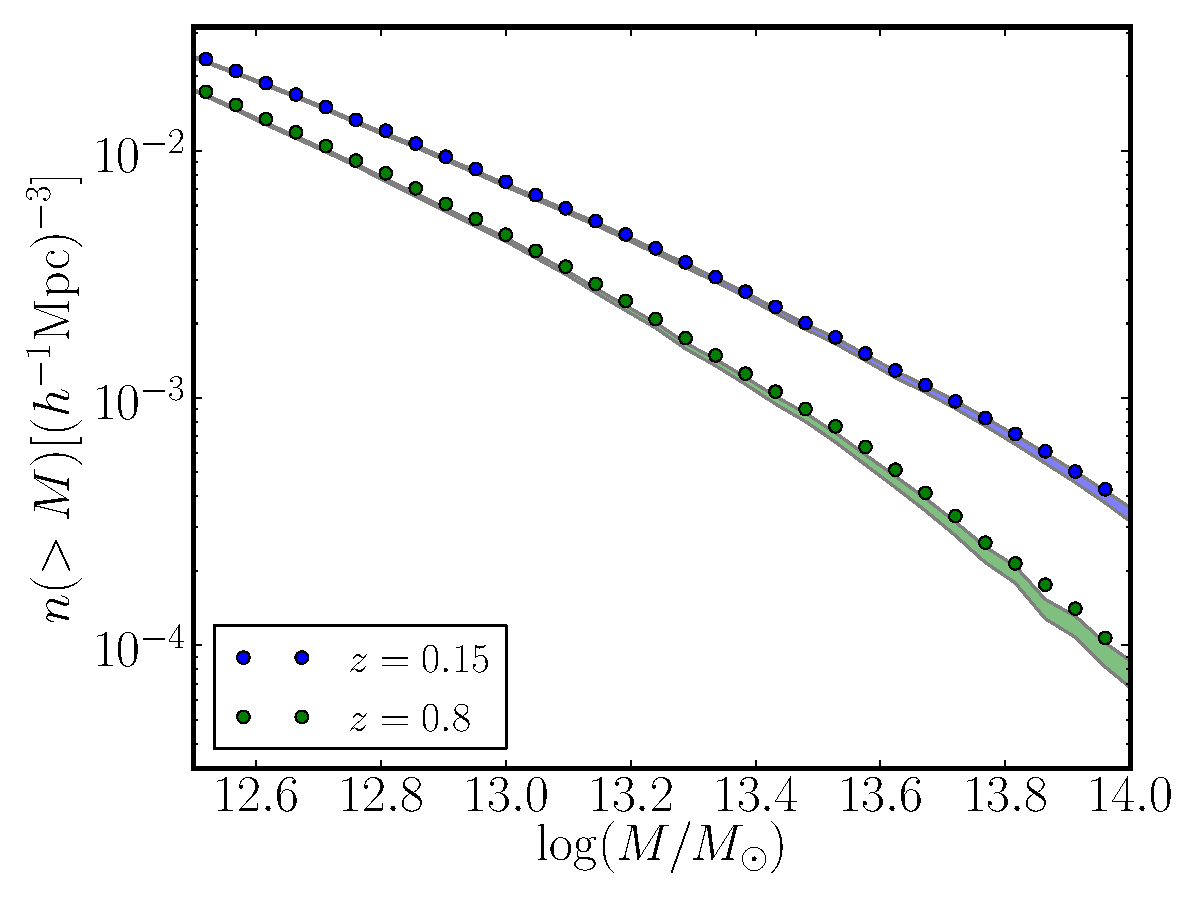
\includegraphics[width=1\columnwidth]{/Users/ts485/Dropbox/Tomomi/HACC/Conv/Plots4lyx/haloNum_massResolution}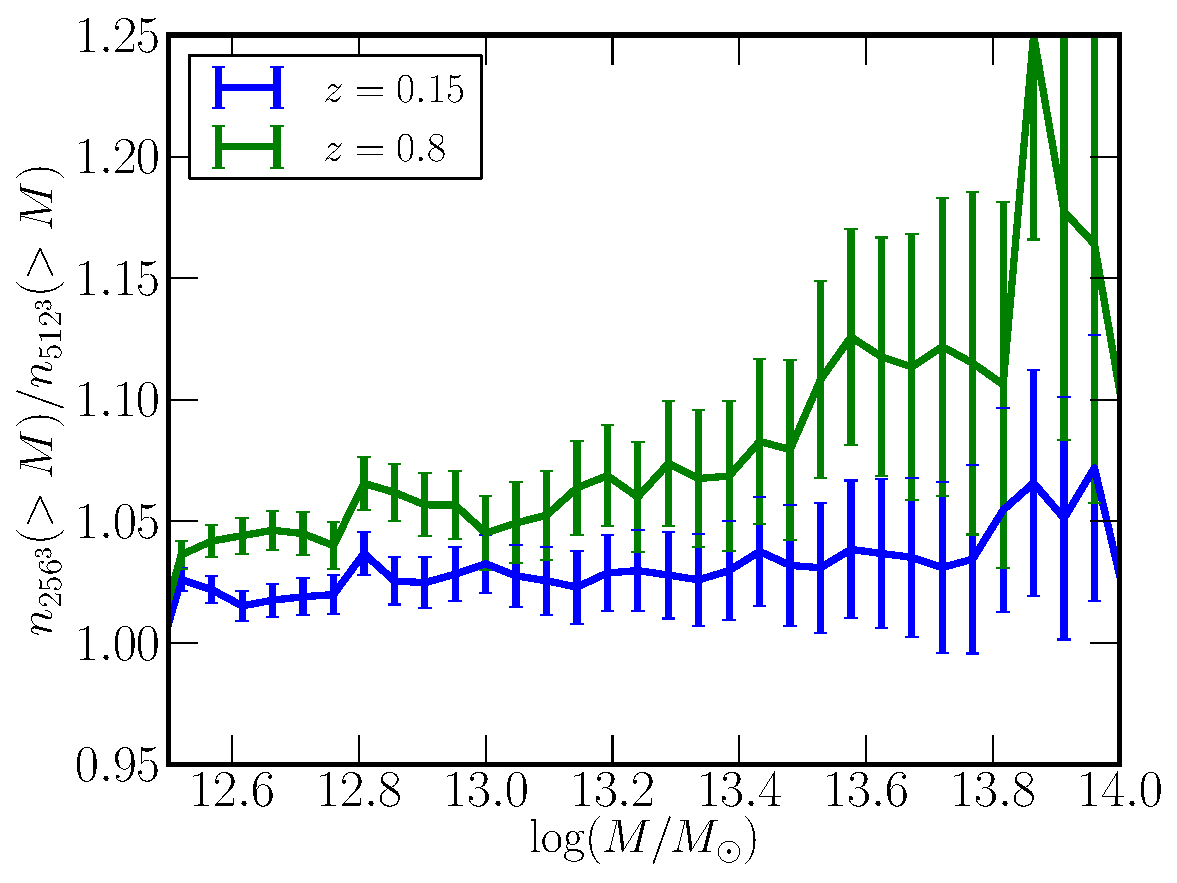
\includegraphics[width=1\columnwidth]{/Users/ts485/Dropbox/Tomomi/HACC/Conv/Plots4lyx/haloRatioNum_massResolution}

\caption{\label{fig:massFn512}Comparison of mass functions (should I call
this number density?) for different simulations at redshift $z=0.15$
and $z=0.8$. The shaded regions indicate the upper limit and the
lower limit of mass functions for the simulation with $512^{3}$ particles
and 450 steps with 5 sub-cycles. The mean and standard deviations
are calculated from bootstrap method. We compare them with the simulations
of $256^{3}$ particles with 450 global steps and 5 sub-cycles (described
as $256^{3}$ with circles in the figure) and $128^{3}$ particles
with 450 global steps and 5 sub-cycles (described as $128^{3}$ with
red stars in the figure). }
\end{figure*}



\subsubsection{Time Steps}

Here, we check the same thing as 2.1.1 for varying time steps with
a fixed mass reslution of $256^{3}$ particles. Figure \ref{fig:massFn256}
compares 450/5 and 300/2 with $512^{3}$ particles mass resolution
and 450/5 time steps. The colored regions indicate number densities
of $512^{3}:450/5$ with errors. Both 450/5 and 300/2 for $256^{3}$
particles are well within the errors. Figure \ref{fig:massFnRatio}
shows the ratios between $512^{3}:450/5$ and $256^{3}$ particles
with different time steps. For the case of 450 and 300 global time
steps, the agreement is better than 10\%.

\begin{figure*}[p]
\includegraphics[width=1\columnwidth]{/Users/ts485/Dropbox/Tomomi/HACC/Conv/Plots4lyx/haloNum2}

\caption{\label{fig:massFn256}Comparison of mass functions (should I call
this number density?) for different simulations at redshift $z=0.15$
and $z=0.8$. The shaded regions indicate the upper limit and the
lower limit of mass functions for the simulation with $512^{3}$ particles
and 450 steps with 5 inner(?) steps. The mean and standard deviations
are calculated from bootstrap method. We compare them with the simulations
of $256^{3}$ particles with 450 global steps and 5 sub-cycles (described
as $256^{3}(450:5)$ with circles in the figure) and with 300 global
steps and 2 sub-cycles (described as $256^{3}(300:2)$ with red stars
in the figure).}


\end{figure*}


\begin{figure*}[p]
\includegraphics[width=1\columnwidth]{/Users/ts485/Dropbox/Tomomi/HACC/Conv/Plots4lyx/haloRatioNum256_z0\lyxdot 15}\caption{\label{fig:massFnRatio}Ratios of mass functions of different time
steps with $256^{3}$ particles, compared to $512^{3}$ particles
with 450 global steps and 5 sub-cycles, at redshift $z=0.15$. Different
colors are corresponding to different time steps. The legend in the
plot has the same format as the one in Figure 1. This plot shows that
the simulations with 450 and 300 global steps agree well with the
simulation with $512^{3}$ particles.}
\end{figure*}



\subsection{Halo power spectra}

In this section, we examine how mass resolution and time steps change
statistical observables (i.e., auto- and cross-power spectra). By
calculating those quantities, we want to know what the smallest global
steps and sub-cycles required to preserve enough properties on power
spectra for observations. 


\subsubsection{Mass Resolution}

In this subsection, we calculate auto power spectra for two different
mass resolutions, $512^{3}$ and $256^{3}$ particles in a $(256h^{-1}{\rm Mpc})^{3}$
cubic box. Halos used here are selected so that those halo masses
are greater than $10^{12.5}{\rm M_{\odot}}$. 

In Figure \ref{fig:autoPower512}, we show various auto power spectra
for $512^{3}$ and $256^{3}$ particles-simulations at redshift $z=0.15$,
$z=0.5$, and $z=0.8$ on the left panels and ratios of auto power
spectra between those two samples on the right panels. Power spectra
on the upper panels are subtracted a Poisson shot noise of $1/n$,
where $n$ is the nuber density of halos. The lower panels are the
same as the upper panels without a Poisson shot noise subtraction.
As shown in Figure \ref{fig:autoPower512}, the agreement between
$512^{3}$ and $256^{3}$ particles- simulations is within 10\%.

\begin{figure*}
\includegraphics[width=1\columnwidth]{/Users/ts485/Dropbox/Tomomi/HACC/Conv/Plots4lyx/autoPower_mcut12\lyxdot 5_ws}
\includegraphics[width=1\columnwidth]{/Users/ts485/Dropbox/Tomomi/HACC/Conv/Plots4lyx/autoPower_ratio_mcut12\lyxdot 5_ws}

\includegraphics[width=1\columnwidth]{/Users/ts485/Dropbox/Tomomi/HACC/Conv/Plots4lyx/autoPower_mcut12\lyxdot 5_wo}\includegraphics[width=1\columnwidth]{/Users/ts485/Dropbox/Tomomi/HACC/Conv/Plots4lyx/autoPower_ratio_mcut12\lyxdot 5_wo}

\caption{\label{fig:autoPower512}Halo auto power spectra for different mass
resolutions ($512^{3}$, $256^{3}$, and $128^{3}$ particles in the
box of $(256h^{-1}{\rm Mpc})^{3}$) with a fixed time step of 450/5.
The sample of halos is equivalent to a mass thresholds of $M=10^{13.5}{\rm M_{\odot}}$.}
\end{figure*}



\subsubsection{Time Steps}

In this subsection, we examine effects of time steps on power spectra.
While global steps is responsible for resolving the large scale structure,
sub-cycles mainly afftes on the small scales and inner structure of
halos\textcolor{black}{. We want to evaluate qualitative effects of
those} differences on dynamics.

In Figure \ref{fig:autoPower_time}, we show various auto power spectra
for 450/5 and 300/2 at redshift $z=0.15$, $z=0.5$, and $z=0.8$
on the left panels and ratios of auto power spectra for different
global steps and sub-cycles at redshift $z=0.15$ on the right panels.
Power spectra on the upper panels are subtracted a Poisson shot noise
of $1/n$, where $n$ is the nuber density of halos. The lower panels
are the same as the upper panels without a Poisson shot noise subtraction.
Note that halos selected here has a mass treshhold of $10^{12.5}{\rm M_{\odot}}$.
As shown in Figure \ref{fig:autoPower_time}, the agreement between
450/5 and other time steps is within 10\%.

\begin{figure*}[t]
\includegraphics[width=1\columnwidth]{/Users/ts485/Dropbox/Tomomi/HACC/Conv/Plots4lyx/autoPower_256_mcut12\lyxdot 5_ws}\includegraphics[width=1\columnwidth]{/Users/ts485/Dropbox/Tomomi/HACC/Conv/Plots4lyx/autoPower_ratio_256_mcut12\lyxdot 5_ws_z0\lyxdot 15}

\includegraphics[width=1\columnwidth]{/Users/ts485/Dropbox/Tomomi/HACC/Conv/Plots4lyx/autoPower_256_mcut12\lyxdot 5_wo}\includegraphics[width=1\columnwidth]{/Users/ts485/Dropbox/Tomomi/HACC/Conv/Plots4lyx/autoPower_ratio_256_mcut12\lyxdot 5_wo_z0\lyxdot 15}

\caption{\label{fig:autoPower_time}Left: Halo auto power spectra for different
redshift $z=0.15$ (blue), $z=0.5$ (green), and $z=0.8$ (red), which
compare 450/5 (dashed line) and 300/2 (circles). Right: Ratios of
halo auto power spectra between 450/5 and other time steps at redshift
$z=0.15$. All the samples used here has the same mass resolution,
$256^{3}$ particles in a $(256h^{-1}{\rm Mpc})^{3}$ cubic box. The
upper panels are subtracted a Poission shot noise, while the lower
panels are without a Poisson shot noise subtraction. The sample of
halos is equivalent to a mass thresholds of $M=10^{12.5}{\rm M_{\odot}}$.}
\end{figure*}


In Figure \ref{fig:crossPower_time}, we computed the cross power
spectra between halos and the matter field at redshift $z=0.15$.
For the matter field, we used the one for $256^{3}$ particles mass
resolution with 450/5 time steps. On the left panel, we show three
different mass bins and compare 300/2 (circles) and 450/5 (solid line)
simulations. They agree remarkably well. On the right panel, we take
ratios between the cross power spectrum for 450/5 time steps and the
cross for other time steps. Halos selected for the right panel has
a mass from $10^{12.5}{\rm M_{\odot}}$ to $10^{13.0}{\rm M_{\odot}}$.
We see that all the ratios are within 5\% accuracy except 150/2 simulations
on small scales. Note that those ratios are equivalent to the ratios
of the halo biases, which implies that biases for different time steps
are almost the same.

\begin{figure*}[p]
\includegraphics[width=1\columnwidth]{/Users/ts485/Dropbox/Tomomi/HACC/Conv/Plots4lyx/crossMatter4_z0\lyxdot 15}\includegraphics[width=1\columnwidth]{/Users/ts485/Dropbox/Tomomi/HACC/Conv/Plots4lyx/crossMatter3_ratio_mcut12\lyxdot 5to13\lyxdot 0_z0\lyxdot 15}

\caption{\label{fig:crossPower_time}Left: Cross power spectra between halos
and DM particles at redshift $z=0.15$. DM particles are taken from
the simulation of $256^{3}$ particles with 450 global steps and 5
sub-cycles. Different colors indicate different halo mass slices:
${\rm log_{10}M\in[12.5,13.0]}$ (blue), ${\rm log_{10}M\in[13.0,13.5]}$
(green), and ${\rm log_{10}M>13.5}$ (red). Lines are the simulations
with 450 global steps and 5 sub-cycles, and circles are the ones with
300 global steps and 2 sub-cycles. Right:Ratios of cross power spectra
for different simulations with respect to the cross power spectra
with 450 global steps and 5 sub-cycles. }


\end{figure*}



\section{Observable Box}

What we want to check/know here are:

1) What redshift can we use linear-shifting?,

2) What redshift-step size is required to preserve dynamics in simulations?


\appendix{Appendix A: snapshots for unmatched halos whose mass is greater than
$10^{14}{\rm M_{\odot}}$. There is a weird case between 450\_5 and
300\_2}

\begin{figure*}[t]
\includegraphics[width=1\textwidth]{/Users/ts485/Dropbox/Tomomi/HACC/Conv/Snap1_256_300_2_z0\lyxdot 15}

\caption{Snapshot of halos between 450/5 and 300/2 which don't agree completey.
All the surrounding halos in 300/2 have distance more than $2h^{-1}{\rm Mpc}$
from an unmatched halo in 450/5.}
\end{figure*}



\appendix{Appendix B: mass selected samples v.s. matched halo samples}
\begin{itemize}
\item Comparison of matched halo samples and mass-sliced samples: what the
comparison indicates is that corresponding halos don't have the same
masses. ->What kind of problems do we have by having this issue?->$b(M)$
may be diffrent for different simulations. 
\end{itemize}
\begin{figure*}
\includegraphics[width=1\columnwidth]{/Users/ts485/Dropbox/Tomomi/HACC/Conv/Plots4lyx/crossCoeff2_mcut12\lyxdot 5to13\lyxdot 0_z0\lyxdot 15}
\includegraphics[width=1\columnwidth]{/Users/ts485/Dropbox/Tomomi/HACC/Conv/matchedCross1_mcut12\lyxdot 5to13\lyxdot 0_z0\lyxdot 15}

\caption{Cross-power coefficients for mass-selected halos (left) and for matched
halos (right) at redshift $z=0.15$. Both cross power coefficients
compare the 450/5 simulation and other time steps. Halos for 450/5
have a mass from $10^{12.5}{\rm M_{\odot}}$ to $10^{13.0}{\rm M_{\odot}}$.}
\end{figure*}


\begin{figure*}
\includegraphics[width=1\columnwidth]{/Users/ts485/Dropbox/Tomomi/HACC/Conv/Plots4lyx/Bias_mass_ws_mcut12\lyxdot 5to13\lyxdot 0_z0\lyxdot 15}\includegraphics[width=1\columnwidth]{/Users/ts485/Dropbox/Tomomi/HACC/Conv/Plots4lyx/Bias_matched_ws_mcut12\lyxdot 5to13\lyxdot 0_z0\lyxdot 15}

\caption{Halo Biases for different stepsizes with $256^{3}$ particles at redshift
$z=0.15$. Left panel is halo biases for samples which are selected
based on mass, and right panel is for samples which are corresponding
to halos of 450 global steps and 5 sub-cycles. Different colors indicate
different stepsizes and mass range for halo samples is from $10^{12.5}{\rm M_{\odot}}$
to $10^{13.0}{\rm M_{\odot}}$.}
\end{figure*}



\appendix{Appendix C: Extra Plots}

\begin{figure*}
\includegraphics[width=1\columnwidth]{/Users/ts485/Dropbox/Tomomi/HACC/Conv/Plots4lyx/autoPower2_256_mcut12\lyxdot 5_ws_mass}

\caption{Auto power spectra for different halo mass bins, which compare 450/5
(solid line) and 300/2 (circles) at redshift $z=0.15$.}
\end{figure*}


\begin{figure*}
\includegraphics[width=1\columnwidth]{/Users/ts485/Dropbox/Tomomi/HACC/Conv/Plots4lyx/crossCoeff2_mcut12\lyxdot 5to13\lyxdot 0_z0\lyxdot 15}

\caption{Cross power coefficients between 450/5 and other time steps at redshift
$z=0.15$. Halos used here have a mass from $10^{12.5}{\rm M_{\odot}}$
to $10^{13.0}{\rm M_{\odot}}$.}
\end{figure*}


\begin{figure}
\includegraphics[width=1\columnwidth]{/Users/ts485/Dropbox/Tomomi/HACC/Conv/Matching_halos/plots_450_5/velMag1_normed_450_5_z0\lyxdot 15}\includegraphics[width=1\columnwidth]{/Users/ts485/Dropbox/Tomomi/HACC/Conv/Plots4lyx/velMag1_normed_450_5_z0\lyxdot 5}\includegraphics[width=1\columnwidth]{/Users/ts485/Dropbox/Tomomi/HACC/Conv/Plots4lyx/velMag1_normed_450_5_z0\lyxdot 8}

\caption{Histograms of velocity magnitude difference for matched halos with
respect to halos from $512^{3}$ particles at redshift $z=0.15$(left),
$z=0.5$ (middle), and $z=0.8$ (right). Different colors correspond
to different mass resolutions: $256^{3}$ particles (blue) and $128^{3}$
particles (green). All the simulations use the same step size, 450/5.
Note that angle difference of velocity vectors for 95\% of matched
halos in the $256^{3}$-particle sample are within 0.3 radians and
90\% in the $128^{3}$-particle sample are within 0.6 radians.}


\end{figure}


\begin{table}
\begin{tabular}{|c|c|c|}
\hline 
$256^{3}$ & mean {[}$km/s${]} & std {[}$km/s${]}\tabularnewline
\hline 
\hline 
$z=0.15$ & 1.69 & 33.60\tabularnewline
\hline 
$z=0.5$ & 7.09 & 49.94\tabularnewline
\hline 
$z=0.8$ & 4.82 & 59.42\tabularnewline
\hline 
\end{tabular}%
\begin{tabular}{|c|c|c|}
\hline 
$128^{3}$ & mean {[}$km/s${]} & std {[}$km/s${]}\tabularnewline
\hline 
\hline 
$z=0.15$ & 9.47 & 59.45\tabularnewline
\hline 
$z=0.5$ & 16.18 & 74.44\tabularnewline
\hline 
$z=0.8$ & 24.97 & 89.64\tabularnewline
\hline 
\end{tabular}

\caption{Mean and standard deviations for the velocity magnitude difference
histograms, which compares $256^{3}/128^{3}$ particles with $512^{3}$
particles. I just felt wierd that deviations on means from 0.0 become
bigger and the values of standard deviations become bigger as redshift
goes higher. I feel that this should be opposite...}


\end{table}

\end{document}
